\mode*

\section{Moduler}

\begin{frame}[fragile]
  \begin{lstlisting}[numbers=none,basicstyle=\huge]
import module
  \end{lstlisting}
\end{frame}

\subsection{Hur?}

\begin{frame}[fragile]
  \begin{example}[bad-module.py]
    \lstinputlisting{examples/bad_module.py}
  \end{example}
\end{frame}

\begin{frame}[fragile]
  \begin{example}[test-good-bad.py]
    \lstinputlisting{examples/test_good_bad.py}
  \end{example}
\end{frame}

\begin{frame}[fragile]
  \begin{example}[good-module.py]
    \lstinputlisting{examples/good_module.py}
  \end{example}
\end{frame}

\subsection{Ett gammalt exempel}

\begin{frame}[fragile]
  \begin{example}[input-type.py, del 1]
    \lstinputlisting[linerange=1-13]{examples/input_type.py}
  \end{example}
\end{frame}

\begin{frame}[fragile]
  \begin{example}[input-type.py, del 2]
    \lstinputlisting[firstline=14,firstnumber=14]{examples/input_type.py}
  \end{example}
\end{frame}

\begin{frame}[fragile]
  \begin{example}[Använda modulen]
    \begin{lstlisting}
import input_type

x = input_type(int, "x = ")
print(f"x = {x}")
    \end{lstlisting}
  \end{example}
\end{frame}


\section{Linting}

\begin{frame}[fragile]
  \begin{lstlisting}[numbers=none,basicstyle=\huge]
$ pylint prog.py
  \end{lstlisting}
\end{frame}

\section{Rekursion}

\begin{frame}[fragile]
  \begin{lstlisting}[basicstyle=\huge,numbers=none]
def f(x):
  if p(x):
    return c
  else:
    return f(g(x))
  \end{lstlisting}
\end{frame}

\subsection{Fakultet}

\begin{frame}[fragile]
  \begin{example}[factorial.py, del 1]
    \lstinputlisting[linerange=1-12]{examples/factorial.py}
  \end{example}
\end{frame}

\begin{frame}[fragile]
  \begin{example}[factorial.py, del 2]
    \lstinputlisting[firstline=12,firstnumber=12]{examples/factorial.py}
  \end{example}
\end{frame}

\subsection{Sökning}

\begin{frame}[fragile]
  \begin{example}[search.py, del 1]
    \lstinputlisting[linerange=5-20,firstnumber=5]{examples/search.py}
  \end{example}
\end{frame}

\begin{frame}[fragile]
  \begin{example}[search.py, del 2]
    \lstinputlisting[linerange=3-3,firstnumber=3]{examples/search.py}
    \dots
    \lstinputlisting[firstline=21,firstnumber=21]{examples/search.py}
  \end{example}
\end{frame}


\section{Generatorer}

\begin{frame}[fragile]
  \begin{lstlisting}[basicstyle=\huge,numbers=none]
def gen():
  i = 0
  while True:
    yield i
    i += 1
  \end{lstlisting}
\end{frame}

\subsection{Filtrering och mappning igen}

\begin{frame}[fragile]
  \begin{example}[filter-own.py]
    \lstinputlisting[linerange=7-12,firstnumber=7]{examples/filter_own.py}
  \end{example}

  \pause

  \begin{example}[filter-gen.py]
    \lstinputlisting[linerange=7-11,firstnumber=7]{examples/filter_gen.py}
  \end{example}
\end{frame}

\begin{frame}[fragile]
  \begin{example}[mapping-own.py]
    \lstinputlisting[linerange=16-20,firstnumber=16]{examples/mapping_own.py}
  \end{example}

  \pause

  \begin{example}[mapping-gen.py]
    \lstinputlisting[linerange=16-20,firstnumber=16]{examples/mapping_gen.py}
  \end{example}
\end{frame}

\subsection{Vad är egentligen skillnaden?}

\begin{frame}[fragile]
  \begin{example}[gen\textunderscore adv.py, del 1]
    \lstinputlisting[linerange=3-13,firstnumber=3]{examples/gen_adv.py}
  \end{example}
\end{frame}

\begin{frame}[fragile]
  \begin{example}[gen\textunderscore adv.py, del 2]
    \lstinputlisting[firstline=15,firstnumber=15]{examples/gen_adv.py}
  \end{example}
\end{frame}


\section{PyPI}

\begin{frame}
  
\includegraphics[width=\columnwidth]{figs/pypi.png}
\end{frame}

\begin{frame}
  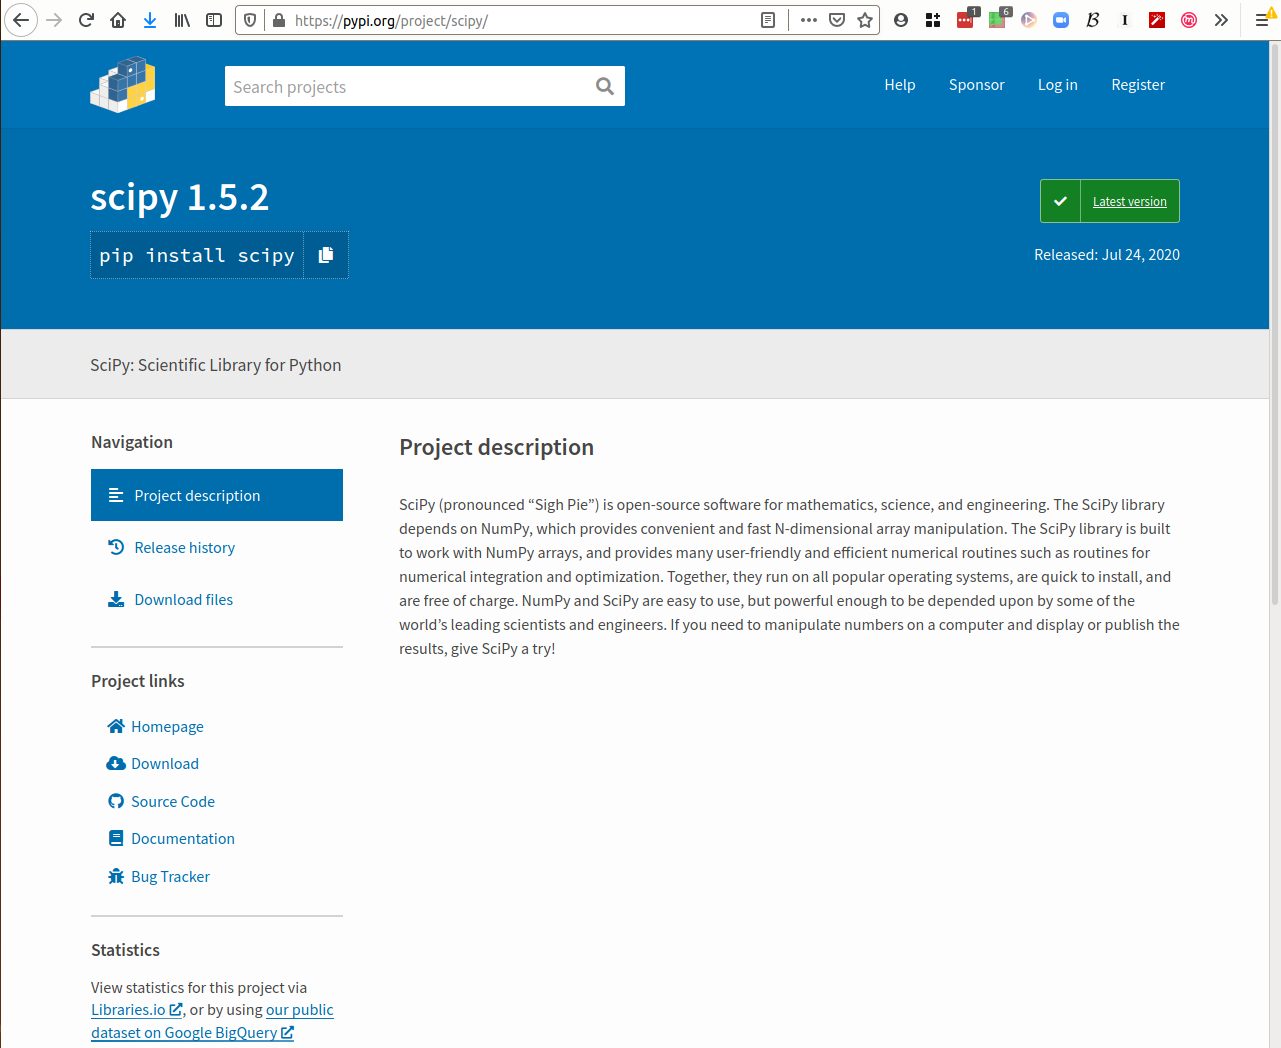
\includegraphics[width=\columnwidth]{figs/pypi-scipy.png}
\end{frame}

\begin{frame}
  
\includegraphics[width=\columnwidth]{figs/pypi-matplotlib.png}
\end{frame}

\begin{frame}[fragile]
  \begin{example}[Installation]
    \begin{lstlisting}[language={},numbers=none]
$ pip install numpy scipy matplotlib
    \end{lstlisting}
  \end{example}
\end{frame}

\begin{frame}
  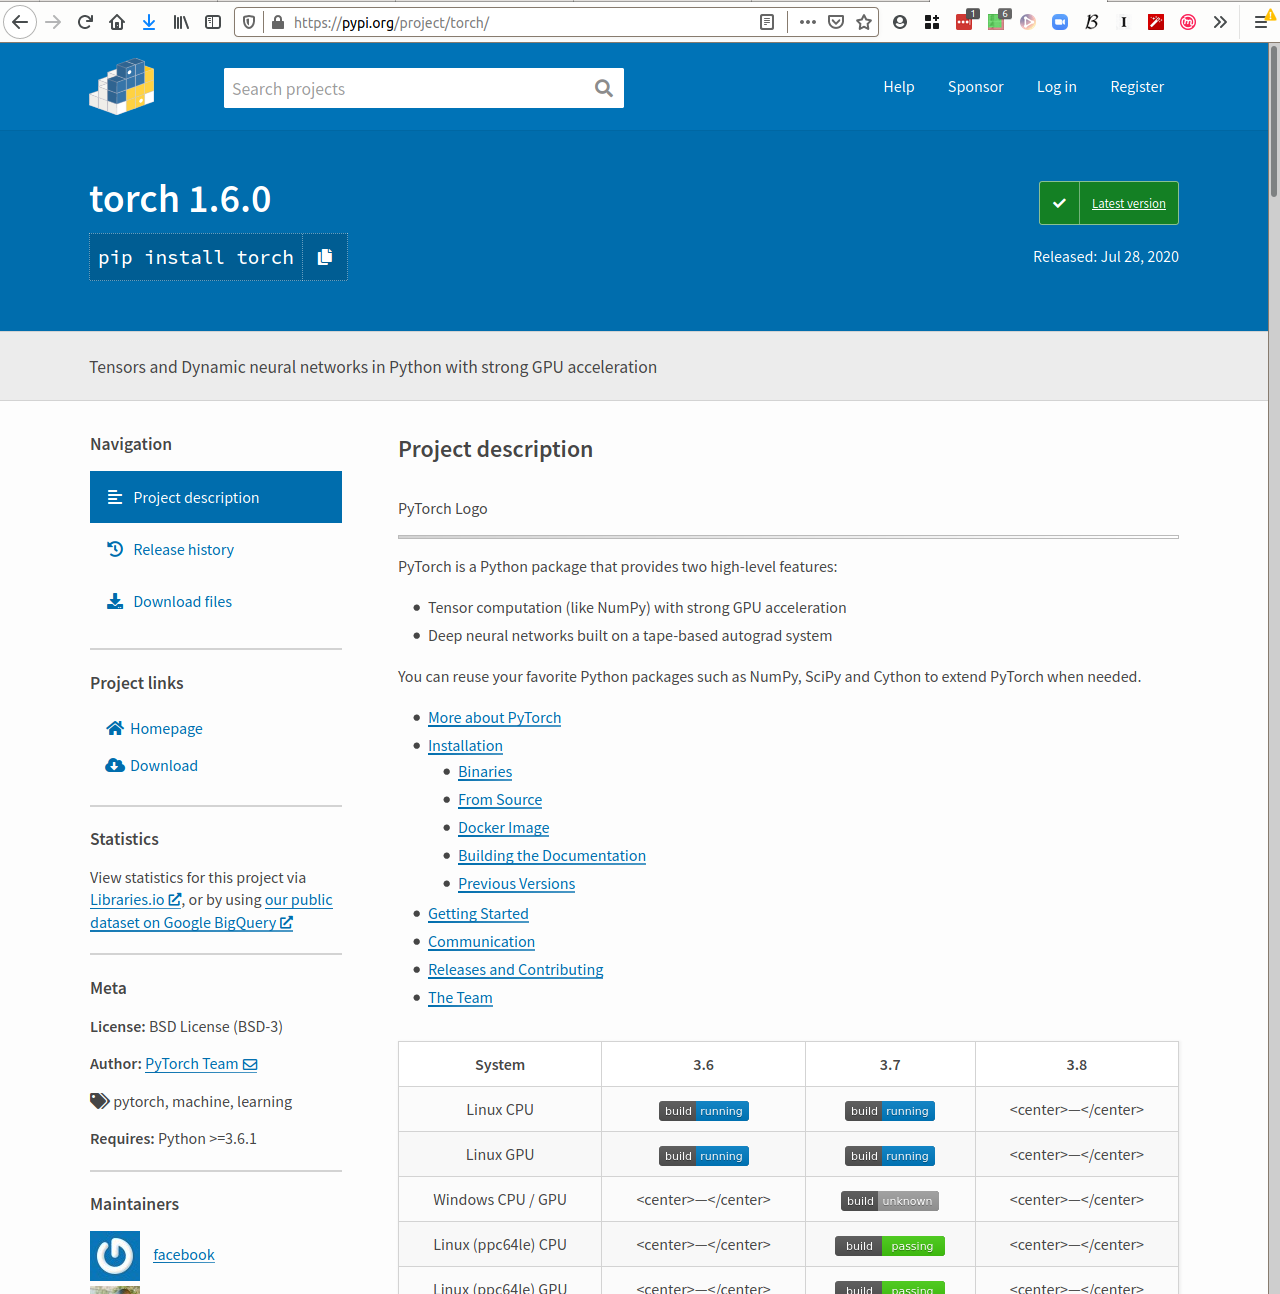
\includegraphics[width=\columnwidth]{figs/pypi-torch.png}
\end{frame}

